
\chapter{Hashes}
\label{hashes}

Este capítulo presenta otro tipo integrado conocido como un
hash. Los hashes son unas de las mejores y más comunes 
características de Perl; ellos constituyen los componentes básicos
de muchos algoritmos eficientes y elegantes.

\section{Un Hash es un Mapeo}
\label{hash_descr}

\index{hash}
\index{type!hash}
\index{key}
\index{key-value pair}
\index{index}
\index{mapping}
Un {\bf hash} es como un array, pero más general. En un array,
los índices o subíndices tienen que ser enteros; en un hash,
pueden ser (casi) cualquier cosa.

Un hash contiene una colección de índices, los cuales se llaman
{\bf claves}, y una colección de valores. 
Cada llave está asociada a un valor único. Una clave y un valor
juntos forman un par (un objeto del tipo Pair), o un {\bf par
clave-valor}. Un hash puede ser visto como una colección de parejas de
clave-valor. Los valores en un hash puede también llamarse artículos o 
elementos, como con los arrays.
\index{item}

En otros lenguajes de programación, los hashes son algunas veces
llamados diccionarios, tablas hash, mapas, o arrays asociativos.

En el lenguaje matemático, un hash representa a un {\bf mapeo}
desde las claves a los valores, así que puedes también decir que cada
clave ``mapea`` a un valor. Como un ejemplo, construiremos un hash
que mapea palabras del inglés al español, y por lo tanto las llaves y
los valores son todos cadenas de texto.

En Perl, el nombre de un hash comienza con el sigilo ``\verb|%|``. Para
crear un nuevo hash, solo decláralo de esta manera:
\index{sigil}
\index{sigil, percent}

\begin{verbatim}
> my %ingAesp;
\end{verbatim}

Esto crea un hash vacío. Para agregar artículos al hash,
puedes usar llaves:
\index{curly bracket}
\index{bracket!curly}
\index{brace}

\begin{verbatim}
> %ingAesp{'one'} = 'uno';
uno
\end{verbatim}
%
Esta línea crea un artículo que relaciona la clave
\verb"'one'" al valor \verb"'uno'".  

Si la clave es una cadena de texto que contiene una sola palabra
(i.e., sin ningún espacio en el medio), existe un atajo más 
idiomático para crear la misma entrada de hash:
\index{idiomatic}

\begin{verbatim}
> %ingAesp<one> = 'uno';
uno
\end{verbatim}
%
Si imprimimos el hash, vemos un par clave-valor con el 
operador constructor de pares \verb|=>| entre la clave y
el valor:
\index{pair constructor}

\begin{verbatim}
> say %ingAesp;
one => uno
\end{verbatim}
%
Este formato de salida es también un formato de entrada.
Por ejemplo, puedes crear un hash nuevo con tres artículos:

\begin{verbatim}
> my %ingAesp = ('one' => 'uno', 'two' => 'dos', 'three' => 'tres');
one => uno, three => tres, two => dos
\end{verbatim}
%

El uso del operador constructor de pares \verb|=>| entre claves y 
valores no es requerido; puedes usar comas tambíen:

\begin{verbatim}
my %ingAesp = ('one', 'uno', 'two', 'dos', 'three', 'tres');
\end{verbatim}
%

Pero el constructor de pares tiene la ventaja de mostrar
gráficamente las relaciones clave-valor. El operador constructor
de pares también hace que el uso de comillas no mandatario
en su lado izquierdo (provisto que la clave sea una cuerda 
de texto sin espacios):

\begin{verbatim}
> my %ingAesp = (one => 'uno', two => 'dos', three => 'tres');
one => uno, three => tres, two => dos
\end{verbatim}
%

También podrías usar una sintaxis de lista más concisa para la
asignación del hash y Perl convertirá felizmente la lista
en un hash, provisto que el número de artículos en la lista 
de entrada sea par:

\begin{verbatim}
> my %ingAesp = <one uno two dos three tres>;
one => uno, three => tres, two => dos
\end{verbatim}
%

Podrías sorprenderte con el resultado. El orden de los
pares clave-valor usualmente no se encuentran en el orden
en el cual lo poblaste. En general, el orden de los artículos
en un hash es impredecible.

Pero eso no es un problema porque los elementos de un hash
nunca son indexados con subíndices enteros. En lugar de esto,
usas las claves para consultar los valores correspondientes:

\begin{verbatim}
> say %ingAesp<two>;
dos
\end{verbatim}
%
La clave \verb"two" siempre mapea al valor \verb|`dos`|
así que el orden de los artículos no importa.

Si la clave no se encuentra en el hash, obtienes un valor 
indefinido:

\begin{verbatim}
> say %ingAesp<four>;
(Any)
\end{verbatim}
%
El método o la función {\tt elems} funciona con los hashes
como con los array; devuelve el número de pares clave-valor:
\index{elems function or method}
\index{function!elems}
\index{elems function or method}
\index{method!elems}


\begin{verbatim}
> say %ingAesp.elems;
3
> say elems %ingAesp
3
\end{verbatim}
%
El adverbio {\tt :exists} también funciona con los hashes 
como con los arrays; te dice si algo aparece como una 
{\em clave} en el hash (aparecer como un valor no es suficiente)
\footnote{Evaluar el valor en un contexto Booleano también 
funcionaría con nuestro ejemplo, pero esto devolvería
algo erróneo cuando la clave existe, pero el valor 
no está definido o por lo contrario evalúa a un valor falso
(por ejemplo, si es igual a {\tt False}, cero, o 
cadena de texto vacía).}:
\index{membership!hash}
\index{exists adverb}
\index{adverb!:exists}

\begin{verbatim}
> %ingAesp<two> :exists;
True
> %ingAesp<four> :exists;
False
\end{verbatim}
%
Para chequear si algo aparece como un valor en un hash, 
puedes usar el método {\tt values}, el cual devuelve una 
colección de valores, y después usar un bucle (o posiblemente 
{\tt grep}) para buscar el artículo:
\index{values function or method}
\index{method!values}
\index{grep}

\begin{verbatim}
my @vals = values %ingAesp;
for @vals -> $value {
    say "¡Encontrado!" if $value eq 'uno';           # -> ¡Encontrado!
}
\end{verbatim}
%
O más concisamente:
\begin{verbatim}
say "¡Encontrado!" if grep {$_ eq 'uno'}, %ingAesp.values;
\end{verbatim}

Dado que {\tt grep}  usa por defecto una coincidencia inteligente, 
esto puede hacerse de una forma aún más concisa:

\begin{verbatim}
say "¡Encontrado!" if grep {'uno'}, %ingAesp.values;  # -> ¡Encontrado!
\end{verbatim}

Cuando se inspecciona los valores, el programa tiene que buscar 
los elementos de la lista en orden (o en secuencia), como en la
Sección~\ref{find}. A medida que la lista se vuelve más larga, 
el tiempo de búsqueda se extiende en proporción directa.
\index{sequential search}
\index{search!sequential}

Por el contrario, cuando se inspecciona las claves, Perl usa
un algoritmo de {\bf hashing} que tiene una propiedad interesante:
toma el mismo monto de tiempo sin importar cuantos artículos
se encuentren en el hash. En otras palabras, funciona bastante 
rápido, comparado con el tamaño de la lista, cuando la lista
que se inspecciona es larga. Ésta es la razón por la cual la
solución al ejercicio de par reverso (Ejercicio~\ref{reverse_pair})
del capítulo anterior usando un hash fue casi tres veces más rápido
que la solución de búsqueda binaria (ver Subsección~\ref{sol_reverse_pair}).

\label{ex_employees}
Como ejercicio, usa la muestra de los datos de empleados del 
array multidimensional  de la Sección~\ref{multidimensional array}
(p.~\pageref{multidimensional array}), organízala en un hash, y 
busca algunos salarios. Pista: no necesitas una estructura 
multidimensional para hacer eso con un hash.
Solución: \ref{sol_ex_employees}


\section{Operaciones Comunes con Hashes}

Ya vimos que para poblar un hash, puedes asignarle una lista 
par. Las cuatros formas sintácticas siguientes son correctas:

\begin{verbatim}
my %primer_trimestre  = ("ene" => 1, "feb" => 2, "mar" => 3);
my %segundo_trimestre = (abr => 4, may => 5, jun => 6);
my %tercer_trimestre  = jul => 7, aug => 8, sep => 9;
my %cuarto_trimestre  = < oct 10 nov 11 dec 12 >;
\end{verbatim}

Para agregar un elemento a un hash, solo asigna el hash con
una clave:

\begin{verbatim}
my %meses = ("ene" => 1, "feb" => 2, "mar" => 3);
%meses{'abr'} = 4;
say %meses;         # -> abr => 4, feb => 2, ene => 1, mar => 3
\end{verbatim}

Recuerda que también puedes hacer lo mismo sin encerrar 
las claves en comillas si usas el operador quote-word con
las comillas angulares (si las claves son cadenas de texto):
\index{quote-word operator}
\index{angle bracket}

\begin{verbatim}
%months<abr> = 4;       # igual que: %meses{'abr'} = 4;
\end{verbatim}

o puedes usar la función {\tt push} con un par:
\index{push function}
\index{function!push}

\begin{verbatim}
> push %meses, (may => 5);
abr => 4, feb => 2, jan => 1, mar => 3, may => 5
> my $nuevo-par = jun => 6
jun => 6
> push %meses, $nuevo-par;
abr => 4, feb => 2, jan => 1, jun => 6, mar => 3, may => 5
\end{verbatim}
%

Usar {\tt push} para agregar un par a un hash no es exactamente lo
mismo que hacer una asignación de hash: si la clave ya existe,
el valor antiguo no es reemplazado por el valor nuevo---en lugar,
ambos valores son colocados en un array (o si el valor antiguo se 
encuentra ya en el array, entonces el valor nuevo se agrega al 
array):

\begin{verbatim}
> push %meses, (jan => '01');
{abr => 4, feb => 2, jan => [1 01], jun => 6, mar => 3, may => 5}
\end{verbatim}

Para chequear si un valor está definido para una clave dada,
usa {\tt defined}:
\index{defined}

\begin{verbatim}
> say True if defined %meses<abr>;
True
\end{verbatim}
%

Para obtener el número de artículos en un hash, usa el 
método {\tt elems}:
\index{elems function or method}

\begin{verbatim}
say %meses.elems;                # -> 6
\end{verbatim}

Para remover un artículo del hash, usa el adverbio {\tt :delete}:
\index{delete adverb}
\index{adverb!:delete}

\begin{verbatim}
> push %meses, (jud => 7);      # ¡Oops, un error!
abr => 4, feb => 2, jan => 1, jud => 7, jun => 6, mar => 3, may => 5
> %meses{'jud'}:delete;         # error removido
7
> say %meses
abr => 4, feb => 2, jan => 1, jun => 6, mar => 3, may => 5
\end{verbatim}

Nota que el adverbio {\tt :delete} también devuelve le valor que
ha sido removido.

Para interar sobre un hash, usa:
To iterate over a hash, use:
\index{kv function or method}
\index{keys function or method}
\index{values function or method}
\index{pairs function or method}

\begin{itemize}
\item {\tt kv} para extraer las claves y los valores intercalados;
\item {\tt keys} para extraer las llaves;
\item {\tt values} para extraer los valores;
\item {\tt pairs} para extraer los pares clave-valor;
\end{itemize}

Por ejemplo:

\begin{verbatim}
> for %meses.kv -> $clave, $val { say "$clave => $val" }
jan => 1
abr => 4
mar => 3
jun => 6
may => 5
feb => 2
> say keys %meses;
(jan abr mar jun may feb)
> say values %meses;
(1 4 3 6 5 2)
> say %meses.pairs;
(jan => 1 abr => 4 mar => 3 jun => 6 may => 5 feb => 2)
\end{verbatim}
%

\section{Un Hash como una Colección de Contadores}
\label{histogram}
\index{counter}

Supón que se te provee con una cadena de texto y quieres contar
el número de apariciones de cada letra. Existen varias maneras
en las que puedes hacer esto:

\begin{itemize}

\item Podrías crear 26 variables, una por cada letra del 
alfabeto. Después podrías travesar la cadena de texto y, por cada
carácter, aumentar el contador correspondiente, probablemente
usando una condicional encadenada grande y fea de 26 partes.

\item Podrías crear un array con 26 elementos. Después podría
convertir cada carácter a un número (usando la función integrada
{\tt ord}), usar el número como un índice en el array, e 
incrementar el contador apropiado.

\item Podrías crear un hash con caracteres como claves y contadores
como los valores correspondientes. La primera vez que ves un carácter,
agregarías un artículo al hash. Después de eso, aumentarías el valor
de un artículo existente.
\end{itemize}

Cada una de estas opciones realiza la misma computación,
pero cada una de ellas implementa la computación en una
manera distinta.
\index{implementation}

Una {\bf implementación} es una manera de realizar una computación;
algunas implementaciones son mejores que otras. Por ejemplo,
una ventaja de la implementación con el hash es que no tenemos
que saber con antelación cuales letras aparecen en la 
cadena de texto y solo tenemos que crear espacio para las letras
que si aparecen.

Aquí se muestra como el código podría lucir:

\begin{verbatim}
sub histograma (Str $cadena) {
    my %histo;
    for $cadena.comb -> $letra {
        %histo{$letra}++;
    }
    return %histo;
}
\end{verbatim}
%
El nombre de la función es {\tt histograma}, el cual es
un término estadístico para una colección de contadores (o frecuencias).
\index{histogram}
\index{frequency}
\index{traversal}
\index{comb function and method}
\index{counter}

La primera línea de la función crea un hash vacío.
El bucle {\tt for} traversa la cadena. Cada vez a través
del bucle, si el carácter \verb|$letra| no está en el hash, Perl
crea un artículo nuevo con la clave \verb|$letra| y fija los 
valores 0 cuando el operador ++, así que el primer valor 
inmediatamente después de eso es 1. Si la \verb|$letra| 
ya se encuentra en el hash, el valor se incrementa.
\index{increment operator}

Así es cómo funciona:

\begin{verbatim}
> say histograma("We all live in a yellow submarine")
W => 1, a => 3, b => 1, e => 4, i => 3, l => 5, (...) y => 1
\end{verbatim}
%
El histograma indica que las letras \verb|`W`| y \verb|`b`|
aparecen solo una vez; \verb|`a`| y \verb|`i`| aparecen
tres veces, \verb|`e`| aparece cuatro veces, etc.

\section{Bucles y Hashes}
\index{hash!looping with}
\index{looping!with hashes}
\index{traversal}

Si usas un hash en una sentencia {\tt for}, el bucle 
traversa los pares del hash:

\begin{verbatim}
> for %ingAesp -> $par { say $par}
two => dos
three => tres
one => uno
\end{verbatim}
%

Hemos nombrado la variable de iteración \verb|$par| para
resaltar más claramente que el programa está iterando
sobre los pares clave-valor (actualmente objetos \verb|Pair|).
Puedes usar los métodos {\tt key} y {\tt value} (nota que
están en singular) para acceder
la clave y valor de un \verb|Pair|. Por ejemplo, para revertir
el orden en el cual cada línea es imprimida:

\begin{verbatim}
> for %ingAesp -> $par { say $par.value ~ " <= " ~ $par.key; }
dos <= two
tres <= three
uno <= one
\end{verbatim}

Otra vez, las claves no estás en un orden particular. Para
travesar las claves ordenadamente, puedes usar las funciones
o métodos {\tt keys} (en plural) y {\tt sort}:
\index{keys function or method}
\index{method!keys}
\index{sort!function or method}
\index{method!sort}

\begin{verbatim}
my %histo = histograma("We all live in a yellow submarine");
for %histo.keys.sort -> $clave {
    say "$clave\t%histo{$clave}";
}
\end{verbatim}



\section{Reverse Lookup}
\label{raise}
\index{hash!lookup}
\index{hash!reverse lookup}
\index{lookup, hash}
\index{reverse lookup, hash}

Dado un hash \verb|%hash| y una clave \verb|$k|, es fácil 
encontrar el valor correspondiente \verb|$val = %hash{$k}|.
Esta operación se conoce como una {\bf búsqueda} y, como ya
mencionamos, esta es bastante rápida hasta cuando el hash
es bien grande.
\index{lookup}
\index{hash lookup}

¿Qué pasa si tienes a \verb|$val| y quieres encontrar a \verb|$k|?
Sucede que tienes tres problemas: primero, podrían existir más
de una clave que mapean al valor \verb|$val|; dependiendo de
la aplicación, podrías elegir una, o tendrías que crear un array 
que las contenga a todas. Segundo, no existe una sintaxis simple
para hacer una {\bf búsqueda inversa}; tienes que hacer la búsqueda.
Tercero, podría consumir mucho tiempo si el hash es largo.

Aquí presentamos una función que toman un valor y devuelve
la primera clave que mapea a ese valor:
\index{reverse lookup}

\begin{verbatim}
sub busqueda-inversa (%hash, $val) { 
    for %hash -> $par { 
        return $par.key if $par.value eq $val;
    }
    return;
}
\end{verbatim}
%
Esta subrutina es otro ejemplo del patrón de búsqueda. 
Si llegamos al final del bucle, eso significa que \verb|$val|
no aparece en el hash como un valor, así que devolvemos un 
valor indefinido (Nil). Aquí, la responsabilidad para reaccionar
a tal situación se deja a la función que hace la llamada. 
Una alternativa es levantar una excepción, la cual tendría
que ser todavía la responsabilidad de la función que hace la
llamada. Sin embargo, dado que la búsqueda directa con la clave
no levanta una excepción pero simplemente devuelve un valor indefinido
cuando la clave no existe, hace sentido que {\tt busqueda-inversa}
tenga el mismo comportamiento cuando el valor no se encuentra.

Este es un ejemplo de una búsqueda inversa exitosa:

\begin{verbatim}
> my %histo = histograma('parrot');
a => 1, o => 1, p => 1, r => 2, t => 1
> my $clave =  busqueda-inversa %histo, "2";
r
\end{verbatim}
%
Y una búsqueda sin éxito:

\begin{verbatim}
> say busqueda-inversa %histo, "3";
Nil
\end{verbatim}
%

Otra forma más concisa de hacer la búsqueda inversa sería
usar {\tt grep} para extraer una lista de valores 
que satisfagan nuestra condición:
\begin{verbatim}
say grep { .value == 2 }, %histo.pairs;   # -> (r => 2)
\end{verbatim}

Otra opción es usar una expresión con la función integrada
{\tt first} para extraer solo el primer para:
\begin{verbatim}
my %histo = histograma('parrot');
say %histo.pairs.first: *.value == 1;      # ->  p => 1
\end{verbatim}

\index{whatever}
Este último ejemplo usa el parámetro \emph{whatever} ``*``
el cual no hemos discutido en este libro todavía. Digamos que,
aquí, el ``*`` quiere decir sucesivamente para cada par del hash
y la función {\tt first} devuelve el primer par que coincide
con la condición del valor (ver 
Sección~\ref{whatever star parameter} para detalles sobre
el parámetro ``*``).

Una búsqueda inversa es mucha más lenta que una búsqueda directa;
si tienes que hacerla constantemente, o si el hash se vuelve grande,
el rendimiento de tu programa sufrirá.
\index{reverse lookup}

\section{Comprobando la Existencia}
\index{existence!testing for}

Una tarea bastante común es determinar sin algo existe o si un valor
dado ya se ha visto en un programa. El uso de un hash es usualmente
la mejor solución porque encontrar si existe una entrada para un valor
dado es muy simple y también muy eficiente: solo necesitas almacenar los
valores que quieres inspeccionar como una entrada de clave, y después 
chequear por su existencia cuando sea necesario.

En tal caso, usualmente el valor no es importante y podrías
colocar cualquier cosa. Es muy común en este caso usar ``1`` como
un valor, pero también podrías almacenar {\tt True} o cualquier
otro valor que desees.

Supón que queremos generar 10 números enteros aleatorios entre 0
y 49, pero queremos asegurarnos que los enteros son únicos. Podemos
usar el método {\tt rand} 10 veces con el rango deseado. Pero la
posibilidad de obtener el mismo número dos veces no es tan
insignificante (ver Ejercicio~\ref{birthdays} sobre la 
paradoja del cumpleaños y su solución (Subsección~\ref{sol_birthdays}) 
para una situación similar). Por ejemplo, al intentar esto:
\index{duplicate!checking}
\index{rand function}

\begin{verbatim}
> my @lista;
[]
> push @list, 50.rand.Int for 1..10;
> say @lista;
[12 25 47 10 19 20 25 42 33 20]
\end{verbatim}

se produjo un valor duplicado en la lista (25) en el primer intento.
Y el segundo intento produjo tres pares de duplicados:

\begin{verbatim}
> say @lista;
[45 29 29 27 12 27 20 5 28 45]
\end{verbatim}

Podemos usar un hash para rechazar cualquier entero aleatorio
generado que ya se haya visto. La siguiente manera sería una forma
de escribir esto en código:
\index{rand function}

\begin{verbatim}
my @lista;
my %visto;
while @lista.elems < 10 {
    my $aleatorio = 50.rand.Int;
    next if %visto{$aleatorio}:exists;
    %visto{$aleatorio} = 1;
    push @lista, $aleatorio;
}
say @lista;
\end{verbatim}

Cada valor entero generado se agrega al hash \verb|%visto| 
y la lista de salida. Pero antes de hacer eso, el entero 
generado se chequea con el hash \verb|%visto| para verificar
que no se ha visto todavía. Cuando el programa finaliza su 
ejecución, la lista contiene 10 enteros únicos y (pseudo)aleatorios.

Lo hicimos paso a paso y mantuvimos dos estructuras de datos 
separadas, el array de salida \verb|@lista| y el hash \verb|%visto|,
para hacer el proceso tan claro como sea posible. Pero si lo piensas,
\verb|@lista| y \verb|%visto| tienen esencialmente el mismo contenido
a cada paso a través del bucle. Realmente no tenemos que mantener un
registro de los mismos datos en dos lugares. Dado que tener un hash
es importante para chequear que los valores de salida son únicos, 
podemos deshacernos de \verb|@lista| y escribir una versión más
concisa y probablemente más idiomática del mismo programa:
\index{idiomatic}
\index{push function}

\begin{verbatim}
my %visto;
while %visto.elems < 10 {
	my $aleatorio = 50.rand.Int;
	push %visto, ($aleatorio => 1) unless %visto{$aleatorio}:exists;
}
say keys %visto;      # -> (39 12 46 27 14 21 4 38 25 47)
\end{verbatim}

Esto puede simplificarse aún más. No es realmente necesario
chequear si el entero generado existe en el hash: si existe,
el elemento antiguo del hash será reemplazado con el nuevo, 
y el hash esencialmente no cambiará. Además, cuando se evalúa
en un contexto numérico escalar, un hash devuelve el número de
sus elementos, así que la invocación {\tt .elems} no es necesaria.
Esta es la nueva versión:
\index{scalar context}
\index{elems function or method}

\begin{verbatim}
my %visto;
%visto{50.rand.Int} = 1 while %visto < 10;
say keys %visto;      # -> (46 19 5 36 33 1 20 45 47 30)
\end{verbatim}

Esta última versión es probable más concisa y más idiomática,
pero esto significa que es mejor. Es perfectamente aceptable
si prefieres la segunda o la primera versión porque la encuentras
más clara. Usa la versión que desees, o tu propia versión modificada
provisto que realice la tarea prevista. Esto es Perl, \emph{
hay más de una forma para hacer algo} (TIMTOWTDI).
\index{TIMTOWTDI}

% Hay más de una forma para hacer algo (HMDUFPHA)

Sin embargo, nota que la versión pura de hash no mantiene el orden
en el cual los números son generados, así que (pseudo)aleatoriedad
podría no ser tan buena.

También nota que Perl tiene una función o método {\tt pick}
para elegir elementos de forma aleatorio de una lista sin 
repetición.
\index{pick function or method}


\section{Las Claves de un Hash son Únicas}

No es posible tener la misma clave en un hash más de una vez.
El intento de mapear un nuevo valor a una clave reemplazará el
valor antiguo con el nuevo. Aquí presentamos un ejemplo de la
creación de un hash con claves duplicadas:
\index{duplicate}

\begin{verbatim}
> my %amigos = (Gabo => 5, Miguel => 6, Salomé => 5, Gabo => 7, Jorge => 3)
Miguel => 6, Jorge => 3, Salomé => 5, Gabo => 7
\end{verbatim}

Dado que dos de nuestros amigos se llaman ``Gabo``,  perdemos los
datos asociados con el primero. Esto es algo con lo cual deberías
cuidadoso: las claves de un hash son únicas, así que perderás algunos
artículos si los datos asociados con tus claves tienen duplicados. 
La siguiente sección mostrará algunas maneras de tratar este posible 
problema.

Pero esta propiedad sobre la singularidad de una clave tiene muchos
aspectos positivos. Por ejemplo, una manera típica de remover los duplicados
de una lista de artículos es asignar los artículos de una lista a las
claves de un hash (el valor no importa); al final del proceso, 
la lista de claves no contiene duplicados:

\begin{verbatim}
> my @array = < a b c d s a z a r e s d z r a >
[a b c d s a z a r e s d z r a]
> my %único = map { $_ => 1 }, @array;
a => 1, b => 1, c => 1, d => 1, e => 1, r => 1, s => 1, z => 1
> my @array_único = keys %único;
[z a e s d c b r]
\end{verbatim}

Como puedes ver, los duplicados han sido removidos del 
array de salida. En ejemplos simples como este, la función
integrada {\tt unique} habría sido suficiente para remover los
duplicados de \verb|@array|, pero dentro de un programa más
complejo, es bien común usar un hash (usualmente llamado \verb|%visto|)
para chequear si un valor ya se ha visto.
\index{unique function}
\index{map}

\section{Hashes and Arrays}
\label{invert}

\index{inverting a hash}
\index{hash!invert}
Inverting a hash can be very easy if it is known that the 
values can happen only once (that they are unique). Consider 
for example a hash mapping months to their number in the year 
(we limit the example to five months for brevity):

\begin{verbatim}
> my %months = jan => 1, feb => 2, mar => 3, abr => 4, may => 5;
abr => 4, feb => 2, jan => 1, mar => 3, may => 5
\end{verbatim}
%

We can transform the key-value pairs into a flat list, 
reverse the list, and assign the reversed list to a new 
hash:

\begin{verbatim}
> my %rev_months = %months.kv.reverse;
1 => jan, 2 => feb, 3 => mar, 4 => abr, 5 => may
\end{verbatim}
\index{kv function or method}
\index{reverse function or method}
%

We now have a new hash mapping month numbers to their names.
This can be very handy if a hash is known to be bijective, but this approach does not work correctly if a value can 
happen more than once: in such a case, some pairs will be 
lost:

\begin{verbatim}
> my %months = jan => 1, january => 1, feb => 2, february => 2;
feb => 2, february => 2, jan => 1, january => 1
> my %rev_months = %months.kv.reverse;
1 => january, 2 => february
\end{verbatim}

Arrays can appear as values in a hash.  For example, if you
are given a hash that maps from letters to frequencies, you
might want to invert it; that is, create a hash that maps
from frequencies to letters.  Since there might be several 
letters with the same frequency, each value in the inverted hash 
should probably be an array of letters.
\index{inverting a hash}
\index{hash!invert}

Here is a function that inverts such a hash:

\begin{verbatim}
sub invert-hash (%in-hash) { 
    my %out-hash; 
    for %in-hash.kv -> $key, $val {
        push %out-hash{$val}, $key; 
    }
    return %out-hash;
}
\end{verbatim}
%
Each time through the loop, a hash item is assigned to the  \verb'$key' and \verb'$val' variables, and \verb'$key' is 
appended to the value \verb'%output-hash' for the \verb'$val' 
key; if that value does not exist yet, it is created. At 
the end of the process, the values of \verb'%output-hash' are 
all anonymous arrays.

Here is an example:

\begin{verbatim}
my %rev-hist = invert-hash histogram 'parrot';
say %rev-hist;
dd %rev-hist;
\end{verbatim}

This will display:

\begin{verbatim}
1 => [p a o t], 2 => [r]
Hash %rev-hist = {"1" => $["p", "a", "o", "t"], "2" => $["r"]}
\end{verbatim}

Notice that the {\tt say} function gives a simple representation 
of the hash data, and that the new {\tt dd} (short for ``data 
dumper'') function used here gives more detailed information. 
{\tt dd} is not very commonly used in normal programs, but 
can be quite useful while debugging a program to display a 
detailed description of a complex data structure 
\footnote{To tell the full truth, {\tt dd} is not standard 
Perl~6, it is a Rakudo-specific debugging feature. A future 
implementation of Perl~6 not based on Rakudo might not have 
it.}.
\index{say function or method}
\index{dd function}

\verb'%output-hash' contains two items (two pairs) whose 
values are anonymous arrays. You can access the second 
element of the first array using the hash value 
\verb'%rev-hist{"1"}' as if it was any ordinary array name, 
with this simple syntax:

\begin{verbatim}
say %rev-hist{"1"}[1];  # -> a
\end{verbatim}


\begin{figure}
\centerline
{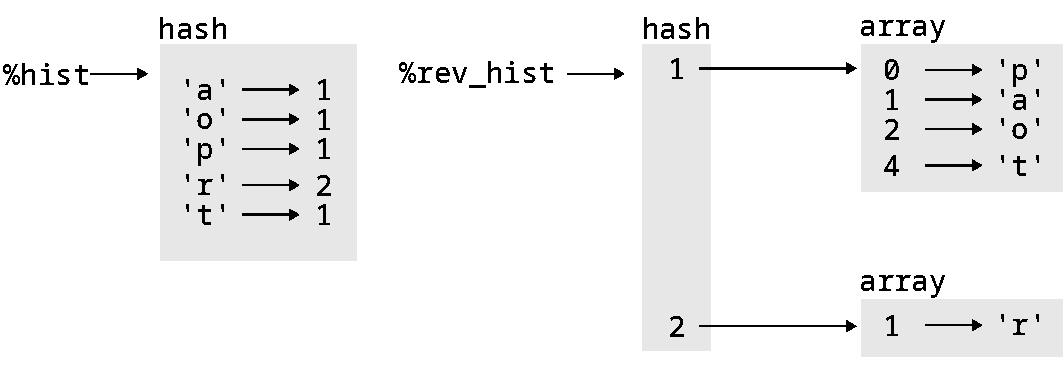
\includegraphics[scale=0.8]{figs/hash1.pdf}}
\caption{State diagram.}
\label{fig.hash1}
\end{figure}

Figure~\ref{fig.hash1} is a state diagram showing \verb'%hist'  and \verb'%rev-hist' .
A hash is represented as a box with the type {\tt hash} above it
and the key-value pairs inside.
\index{state diagram}
\index{diagram!state}

Arrays can be values in a hash, as this example shows, but they
cannot be keys.  If you try, you're likely to end up with a 
key that contains only one item of the array, but most likely 
not what you intended:

\begin{verbatim}
my @a = 'a' .. 'c';
my %h;
%h{@a} = 5;
say %h;  # -> a => 5, b => (Any), c => (Any)
\end{verbatim}

Here, Perl interpreted the \verb'%h{@a} = 5;' assignment 
as a a slice assignment, i.e., assumed that we were 
trying to populate three items in one go, one for each 
element of the array.

\index{hash!function}
\index{hashable}
As mentioned earlier, a hash is implemented using
a hashing function and that means that the keys have to 
be \emph{hashable} \footnote{This is not entirely true. The 
keys of a ``normal'' hash must be hashable and therefore 
immutable. There is another type of hash, object hashes, 
for which the need to have immutable keys does not apply.}. 
A {\bf hashing} is a function that takes 
a value (of any kind) and returns an integer.  Hashes use 
these integers, called hash values, to store and look up 
key-value pairs.
\index{immutability}

This system works fine if the keys are immutable.  But if the
keys are mutable, like with arrays, bad things would happen. For example,
when you create a key-value pair, Perl would hash the key and 
store it in the corresponding location.  If you modify the
key and then hash it again, it would go to a different location.
In that case, you might have two entries for the same key,
or you might not be able to find a key.  Either way, the
hash wouldn't work correctly.

That's why keys have to be hashable, and why mutable types like
arrays aren't. So Perl will do something else that can be 
useful (such as creating three distinct hash items in the 
example above), but will not hash the array itself.

Since hashes are mutable, they can't be used as keys,
but they {\em can} be used as values, so that you can 
have nested hashes.

\section{Memos}
\label{memoize}
\index{memoize}
\index{cache}
\index{memo}
\index{Fibonacci}

If you played with the {\tt fibonacci} subroutine from
Section~\ref{one.more.example}, you might have noticed that 
the bigger the argument you provide, the longer the 
subroutine takes to run. Furthermore, the run time 
increases extremely quickly.
\index{Fibonacci!function}
\index{function!Fibonacci}

To understand why, consider Figure~\ref{fig.fibonacci}, which shows
the {\bf call graph} for {\tt fibonacci} with {\tt n=4}.

\begin{figure}
\centerline
{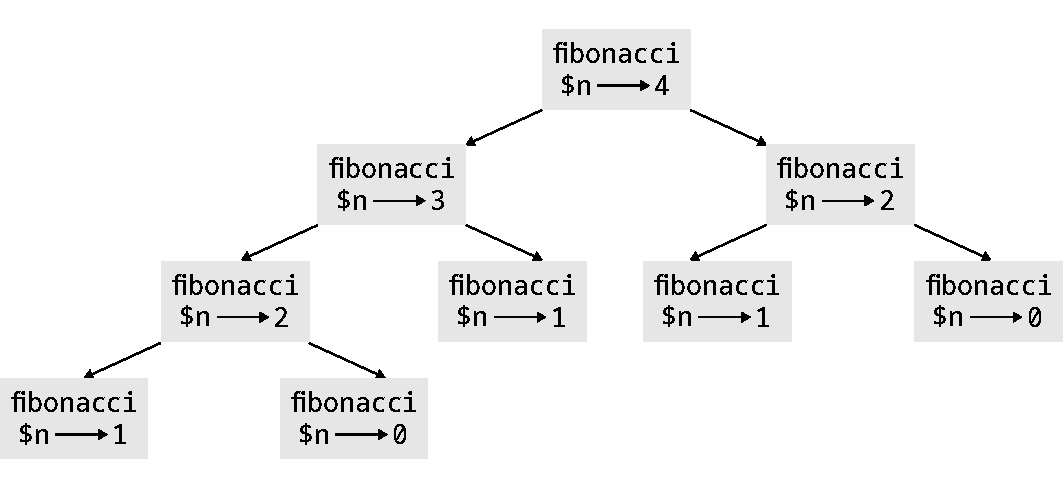
\includegraphics[scale=0.7]{figs/fibonacci.pdf}}
\caption{Call graph.}
\label{fig.fibonacci}
\end{figure}

A call graph shows a set of subroutine frames, with lines 
connecting each frame to the frames of the functions it 
calls.  At the top of the graph, {\tt fibonacci} with 
\verb'$n=4' calls {\tt fibonacci} with \verb'$n=3' and 
\verb'$n=2'.  In turn, {\tt fibonacci} with \verb'$n=3' calls
{\tt fibonacci} with \verb'$n=2' and \verb'$n=1'.  And so on.
\index{function frame}
\index{frame}
\index{call graph}

Count how many times {\tt fibonacci(0)} and {\tt fibonacci(1)} 
are called.  This is an inefficient solution to the problem, 
and it gets much worse as the argument gets bigger.
\index{memo}

One solution is to keep track of values that have already been
computed by storing them in a hash.  A previously computed value
that is stored for later use is called a {\bf memo}.  Here is a
``memoized'' version of {\tt fibonacci}:
\index{Fibonacci!memoized}

\begin{verbatim}
my %known = 0 => 1, 1 => 1;
say fibonacci(10);
sub fibonacci ($n) {
    return %known{$n} if %known{$n}:exists;
    %known{$n} = fibonacci($n-1) + fibonacci($n-2);
    return %known{$n};
}
\end{verbatim}
%

\verb'%known' is a hash that keeps track of the Fibonacci
numbers we already know.  It starts with
two items: 0 and 1, which both map to 1.

Whenever {\tt fibonacci} is called, it checks \verb'%known'.
If the result is already there, it can return
immediately.  Otherwise, it has to 
compute the new value, add it to the hash, and return it.

If you run this version of {\tt fibonacci} and compare it with
the original, you will find that it is much faster, especially 
for a large argument (say more than 30).

\index{cache}
\index{memoize}
Memoizing is a form of \emph{caching}, i.e., storing in memory 
the result of a (presumably costly) computing operation in 
order to avoid computing it again. This process is 
sometimes called ``trading memory against CPU cycles.''  In 
some cases, such as our Fibonacci recursive example here, the gain 
can be absolutely huge: calculating the 100th Fibonacci 
number would take billions of years with the original recursive 
subroutine and it takes only a split second with the memoized 
version.

Please note that in the specific case of the Fibonacci function, 
we are storing values for each successive integer; we could 
have memoized the Fibonacci numbers in an array rather than 
in a hash (and it might even be slightly more efficient), but 
using a hash for such purpose is a more general solution, 
working even when the memo keys are not consecutive integers.

As an exercise, try to rewrite the {\tt fibonacci} subroutine 
using an array instead of a hash to memoize the calculated 
Fibonacci numbers.


\section{Hashes as Dispatch Tables}
\label{dispatch}

You may 
need a procedure to launch some action depending on the 
value of a parameter received by the program. To do that, 
you could use a series of 
\verb'if {...} elsif {...} else {...}' 
statements like this:

\begin{verbatim}
sub run-stop  { ... };
sub run-start { ... };
my $param = get-param;
if $param eq "stop" {
    run-stop;
} elsif $param eq "start" {
    run-start;
} elsif $param = "h" {
    say $help;
} elsif $param = "help" {
    say $help;
} elsif $param = "v" {
    $verbose = True;
} else {
    die "Unknown option $param";
}
\end{verbatim}

This approach is boring and error-prone. Using a dispatch table 
is often a simpler solution.

A dispatch table is a data structure mapping identifiers to 
code references or subroutine objects. Applied to the 
above scenario, it could look like this:

\begin{verbatim}
sub run-stop  { ... };
sub run-start { ... };
my %dispatch = (
    stop  => &run-stop,
    start => &run-start,
    h     => { say $help; },
    help  => { say $help; },
    v     => { $verbose = True;},
);
my $param = get-param();
die "Unknown option $param" unless %dispatch{$param}:exists;
%dispatch{$param}(); # execute the action specified in %dispatch
\end{verbatim}

The \verb'%dispatch' hash defines the action depending on 
the parameter used as a key. The \verb'%dispatch{$param}()' 
statement calls the required action.

This approach is a bit more concise and slightly cleaner, but there 
are some other advantages. It is more maintainable: if you need 
to add one option, you just need to add one entry to the hash 
and don't have to add code in the middle of a complicated 
chain of nested \verb'if {...} elsif {...} else {...}' 
statements at the risk of breaking up something. 

Another upside is that the dispatch table can be dynamically 
modified at run time, for example depending on certain 
external circumstances (for example the day in the month when 
the program is running) or in accordance with a configuration 
file. This means that it is possible to dynamically modify 
the behavior of a program after compile time, while it is 
already running. This paves the way to some very interesting 
advanced programming techniques that are beyond the scope 
of this book.

Note that we have been using hashes for our dispatch tables, 
and this is the most common way to implement them. If it 
makes sense to have small integers as keys, you could also 
implement a dispatch table as an array. This is the case, 
for example, with numbered menu items where the user is 
prompted to type a number to indicate which menu option 
to activate.


\section{Global Variables}
\index{global variable}
\index{variable!global}
\index{lexical variable}
\index{variable!lexical}

In the memoized Fibonacci example above, the 
\verb'%known' hash is created outside the subroutine,
so it belongs to the whole main package.
Such variables are sometimes called {\bf global} 
because they can be accessed from any function.  Unlike ``local'' 
lexical variables, which usually disappear when their scope 
ends, global variables persist from one subroutine call to 
the next.
\index{flag}

It is common to use global variables for {\bf flags}; that is, 
boolean variables that indicate (``flag'') whether a condition
is true.  For example, some programs use a flag named 
\verb'$verbose' to control the level of detail in the
output:

\begin{verbatim}
my $verbose = True;
sub example1 {
    say 'Running example1' if $verbose;
    # ...
}
\end{verbatim}
%

Global variables are also sometimes used for environment 
variables and parameters passed to the program, as well
as for storing a large 
data structure that is the centerpiece of a program, in order 
to avoid copying it when passing it around as an argument to 
subroutines.

But, asides from those specific cases, it is usually 
considered poor practice to use a global variable, because 
it creates dependencies and unexpected ``action-at-a-distance'' 
behaviors between various parts of a program and may lead to 
difficult-to-track bugs.

In the case of our memoized \verb'fibonacci' subroutine, the 
\verb'%known' hash is useful only within the subroutine. We 
can improve the implementation by using the \verb'state' 
declarator within the subroutine:
\index{state}
\index{Fibonacci!memoized with a state variable}

\begin{verbatim}
say fibonacci(10);
sub fibonacci ($n) {
    state %known = 0 => 1, 1 => 1;
    return %known{$n} if %known{$n}:exists;
    %known{$n} = fibonacci($n-1) + fibonacci($n-2);
    return %known{$n};
}
\end{verbatim}
%
The \verb'state' declarator makes the variable local to the 
subroutine and persistent from one call to the subroutine to 
another: the code line with the \verb'state' statement is 
executed only once (at the first call of the subroutine) 
and the content of variable, the \verb'%known' hash in this 
case, is kept from one call to the next.



\section{Debugging}
\index{debugging}

As you work with bigger datasets it can become unwieldy to
debug by printing and checking the output by hand.  Here are some
suggestions for debugging large data sets:

\begin{description}

\item[Scale down the input] If possible, reduce the size of the
dataset.  For example if the program reads a text file, start with
just the first 10 lines, or with the smallest example you can find.
You can either edit the files themselves, or (better) modify the
program so it reads only the first {\tt n} lines.

If there is an error, you can reduce {\tt n} to the smallest
value that manifests the error, and then increase it gradually
as you find and correct errors.

\item[Check summaries and types] Instead of printing and checking the
entire dataset, consider printing summaries of the data: for example,
the number of items in a hash or the total of a list of numbers.

A common cause of runtime errors is a value that is not the right
type.  For debugging this kind of error, it is often enough to print
the type of a value (think about the {\tt .WHAT} method).
\index{WHAT}

It is often useful to add typing to your variables. Where you 
expect a string, make sure you type the variable or subroutine 
parameter with {\tt Str}. If you expect an integer, type it with 
{\tt Int}. If you expect an {\tt Int} of a certain range, create 
a subset for it as in Section~\ref{guardian} (p.~\pageref{guardian}) 
and type the variable with that.
\index{subset!type}
\index{type subset}

\item[Write self-checks:]  Sometimes you can write code to check
for errors automatically.  For example, if you are computing the
average of a list of numbers, you could check that the result is
not greater than the largest element in the list or less than
the smallest.  This is called a ``sanity check'' because it detects
results that are ``insane.''
\index{sanity check}
\index{consistency check}

Another kind of check compares the results of two different
computations to see if they are consistent.  This is called a
``consistency check.''

\item[Format the output] Formatting debugging output
can make it easier to spot an error.  We saw an example in
Section~\ref{factdebug}.  The {\tt dd} function displays 
helpful details on a composite or complex data structure.

\index{dd function}
\index{function!dd}

\end{description}

Again, time you spend building scaffolding can reduce
the time you spend debugging.
\index{scaffolding}


\section{Glossary}

\begin{description}

\item[Mapeo] Una relación en la cual cada elemento de un
conjunto corresponde a un elemento de otro.
\index{mapping}

\item[Hash] Un mapeo de las claves a sus valores correspondientes.
\index{hash}

\item[Par clave-valor] La representación de un mapeo de una sola clave
a su valor.
\index{key-value pair}

\item[Artículos] En un hash, otro nombre para un par clave-valor.
\index{item!hash}

\item[Clave] Un objeto que aparece en un hash como la primera parte
de un par clave-valor.
\index{key}

\item[Valor] Un objeto en un hash que aparece como la segunda parte de 
un par clave-valor. Esto es más específico que nuestro uso previo de
la palabra ``valor``.
\index{value}

\item[Implementación] Una forma de realizar una computación.
\index{implementation}

\item[Tabla hash] El algoritmo usado para implementa hashes.
\index{hashtable}

\item[Función hash] Una función usada por una tabla hash para computar
la ubicación de una clave.
\index{hash!function}

\item[Hashable] Un tipo que contiene una función hash. Los tipos inmutables
como los números y las cadenas de texto son hashables; los tipos
mutables como los array y los hashes no lo son.
\index{hashable}

\item[Búsqueda] Una operación de un hash que toma una clave y encuentra
el valor correspondiente.
\index{lookup}

\item[Búsqueda inversa] Una operación de un hash que toma un valor 
y encuentra una o más claves que mapean al valor.
\index{reverse lookup}

\item[Gráfica de llamada] Una diagrama que muestra cada marco creado 
durante la ejecución de un programa, con una flecha de cada función
que hace la llamada a la función que se llama.
\index{call graph}
\index{diagram!call graph}

\item[Memo] Un valor que se calcula para evitar computaciones futuras
innecesarias.
\index{memo}

\item[Memoizar] Almacenar un valor calculado en la memoria para
evitar cálculos posteriores del mismo. La memoización es una forma
de caché.
\index{memoize}

\item[Variable global]  Una variable definida fuera de cualquier subrutina
u otro bloque. Las variables globales pueden accederse desde cualquier
subrutina.
\index{global variable}

\item[Flag] Una variable Booleana que se usa para indicar si una 
condición es verdadera.
\index{flag}

\end{description}


\section{Ejercicios}

\begin{exercise}
\label{wordlist2}
\index{set!membership}
\index{membership!set}

Escribe una subrutina que lea las palabras en \emph{words.txt}
y las almacene como claves de un hash. (No importa cuales sean los
valores.) Después puedes usar el adverbio {\tt exists} como una manera
rápida de chequear si una cadena de texto se encuentra en el hash.

Si hiciste el Ejercicio~\ref{bisection}, puedes computar la
rapidez de esta implementación con un hash y la búsqueda binaria.

Solución: \ref{sol_wordlist2}

\end{exercise}


\begin{exercise}
\label{mem_ackerman}
Memoiza la función Ackermann del Ejercicio~\ref{ackermann}
y observa si la memoización hace posible evaluar la subrutina
con argumentos más grandes. Pista: no.
Solución: \ref{sol_mem_ackerman}.
\index{Ackermann function}
\index{function!ack}

\end{exercise}



\begin{exercise}
\index{duplicate}
\label{has_duplicates_hash}

Si hiciste el Ejercicio~\ref{has_duplicates}, ya tienes una función
llamada \verb|tiene-duplicados| que toma una lista como un 
parámetro y devuelve {\tt True} si cualquier objeto aparece más
de una vez en la lista.

Usa un hash para escribir un versión más rápida y simple
de \verb|tiene-duplicados|.
Solución: \ref{sol_has_duplicates_hash}.

\end{exercise}


\begin{exercise}
\label{exrotatepairs}
\index{letter rotation}
\index{rotation, letters}

Dos palabras son ``pares rotativos`` si puedes rotar una de ellas
y conseguir la otra (ver \verb"rotar-palabra" en 
Ejercicio~\ref{rotate}) usando el cifrado César.
\index{Caesar cipher}

Escribe un programa que una lista de palabras (por ejemplo, {\tt words.txt}
y encuentre todos los pares rotativos.
Solución: \ref{sol_exrotatepairs}.

\end{exercise}


\begin{exercise}
\label{homophones}
\index{Car Talk}
\index{Puzzler}

Este es otro Puzzler de {\em Car Talk} 
(\url{http://www.cartalk.com/content/puzzlers}):

\begin{quote}

Esto fue enviado por una persona llamada Dan O'Leary. Recientemente,
él encontró una palabra monosilábica de cinco letras que tiene la 
siguiente propiedad única. Cuando se remueve la primera letra, las 
letras restantes forman un homófona de la palabra original, es decir,
una palabra que suena exactamente igual. Reemplaza la primera letra,
es decir, colócala devuelta y remueve la segunda letra y el resultado
es aún otra homófona de la palabra original. Y la pregunta es, cuál es
la palabra?

Ahora te daré un ejemplo que no funciona. Miremos a la palabra de cinco
letras, `wrack`. W-R-A-C-K, como en `wrack with pain'. Si remuevo la primera
letra, me quedo con una palabra de cuatro letras, 'R-A-C-K'. Como en, 
`Holy cow, did you see the rack on that buck!It must have been a nine-pointer!' 
Es un homófono perfecto. Si pones la `w` devuelta, y remueve la `r`, te quedas
con la palabra `wack`, la cual es una palabra real, es solamente no una homófona de
las otras dos palabras.

Pero existe, sin embargo, por lo menos una palabra que Dan y todos
nosotros conocemos, que producirá dos homófonas si remueve una de las primeras
dos letras para crear dos nuevas palabras de cuatro letras. La pregunta es,
cuál es la palabra?
\end{quote}
\index{homophone}
\index{reducible word}
\index{word, reducible}

Puedes usar el hash del Ejercicio~\ref{wordlist2} más arriba para
chequear si una cadena de texto se encuentra {\tt words.txt}.

Para chequear si dos palabras son homófonas, puedes usar el 
Diccionario de Pronunciación CMU. Puedes descargarlo de 
\url{http://www.speech.cs.cmu.edu/cgi-bin/cmudict}.
\index{CMU Pronouncing Dictionary}

Escribe un programa que enumere todas las palabras en {\tt words.txt}
(o en el diccionario CMU) que resuelva el Puzzler.
Solución: \ref{sol_homophones}.

\end{exercise}


